\chapter{Конструкторская часть}
В этом разделе будут приведены требования к ПО, схемы реализации алгоритмов,
а также выбранные классы эквивалентности для тестирования ПО.

\section{Требования к ПО}
Ниже будет представлен список требований к разрабатываемому программному обеспечению. 

Требования к входным данным: 
\begin{itemize}
	\item элементы матрицы должны быть целыми числами;
	\item хотя бы один из линейных размеров матрицы может быть нулевым.
\end{itemize}

Требования к выводу: 
\begin{itemize}
	\item программа должна выводить результирующую матрицу после умножения.
\end{itemize}

\section{Схемы алгоритмов}
На рисунке 2.1 будет приведена схема реализации алгоритма классического умножения матриц.
На рисунках 2.2 будет приведена схема реализации алгоритма Винограда.
На рисунке 2.3 будет приведена схема реализации оптимизированного алгоритма Винограда.

\FloatBarrier
\begin{figure}[hp]
	\begin{center}
		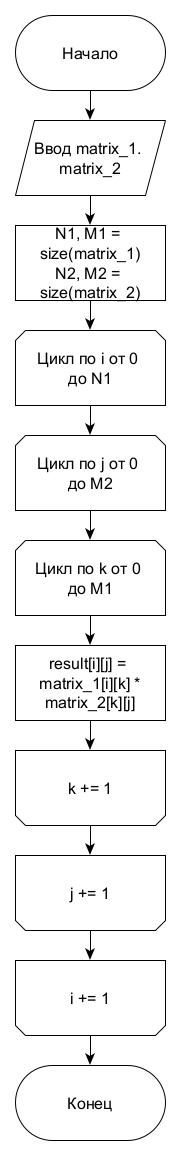
\includegraphics[height=23cm]{graph/classic.jpg}
	\end{center}
	\caption{Схема алгоритма классического умножения матриц}
\end{figure}
\FloatBarrier

\FloatBarrier
\begin{figure}[hp]
	\begin{center}
		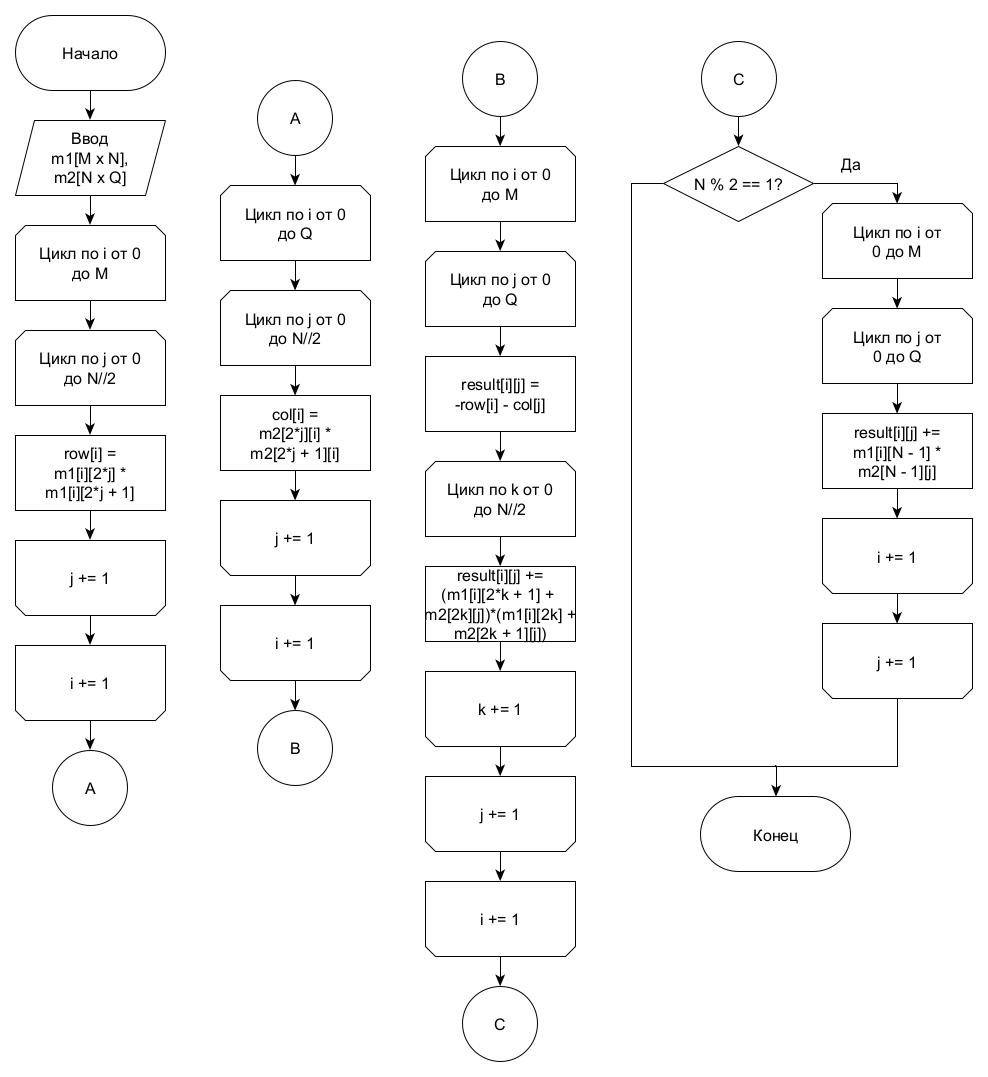
\includegraphics[width=\linewidth]{graph/vinograd.jpg}
	\end{center}
	\caption{Схема алгоритма Винограда}
\end{figure}
\FloatBarrier

\FloatBarrier
\begin{figure}[hp]
	\begin{center}
		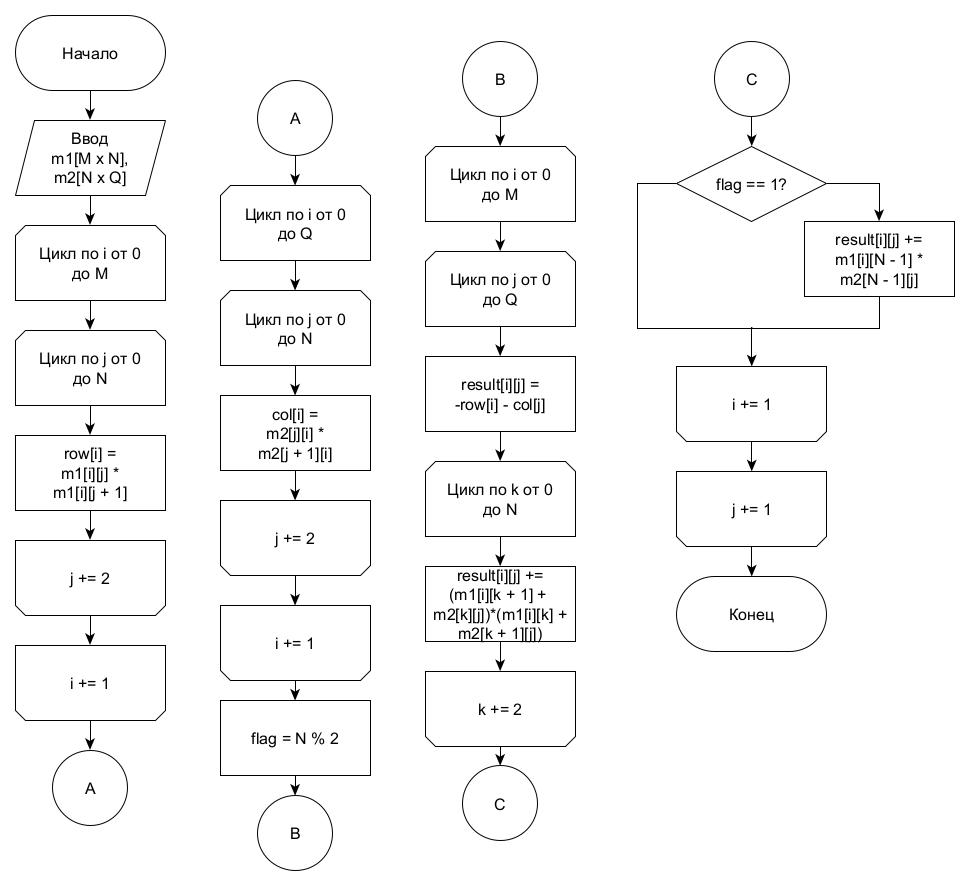
\includegraphics[width=\linewidth]{graph/optvinograd.jpg}
	\end{center}
	\caption{Схема оптимизированного алгоритма Винограда}
\end{figure}
\FloatBarrier

\section{Типы данных для алгоритмов}
Тестирование алгоритмов будет производиться на целых числах, 
которые могут быть и отрицательными, и равны нулю. Несмотря на это,
сами реализации алгоритмов универсальны и предназначены для любых численных типов данных.

Размер матрицы может быть произвольным.

\section{Способ тестирования}
Тестирование программы будет произодиться методом чёрного ящика.
Такой подход выбран, так как от реализаций алгоритмов требуется в первую
очередь правильность работы.
Сама по себе реализация не требует тестировки, так как в точности
повторяет теоретические принципы, сформированные в аналитическом
разделе.

В качестве классов эквивалентности были выбраны следующие сущности:
\begin{itemize}
	\item одна из матриц нулевого размера;
	\item матрицы не соответствуют друг другу по размеру;
	\item матрицы размером в $1 \times 1$;
	\item чётные размеры матрицы;
	\item нечётные размеры матрицы;
	\item одна из матриц - единичная;
	\item одна из матриц - нулевая;
\end{itemize}

Для корректного сравнения требуется для каждой реализации умножения матриц
сравнить полученный на выходе результат с эталонным.

\section{Вывод}
Были приведены требования к ПО, схемы реализации алгоритмов.
Были определен способ тестирования алгоритмов.